\section{Lezione 10 - Reti neurali 2}\label{lezione-10---reti-neurali-2}

Perceptron va bene ma non riesce ad apprendere la XOR perché non è
linearmente separabile.

\subsection{Reti di Perceptron}\label{reti-di-perceptron}

L'idea è quindi quella di combinare più Perceptron tra loro, in modo che
riescano ad apprendere una qualsiasi funzione boolena.

Il problema ora diventa come effettuare l'apprendimento con una rete di
Perceptron, dal momento che non è più triviale come assegnare dei pesi
alle unità nascoste. Una possibile soluzione è quella di rendere il
singolo neurone derivabile e sfruttare la tecnica di Discesa del
Gradiente per apprendere i pesi ``giusti''.

\subsubsection{Discesa di gradiente}\label{discesa-di-gradiente}

\textbf{Richiami di analisi}: il segno della derivata di una funzione
determina se la funzione è crescente o decrescente. Inoltre se la
derviata vale 0, la funzione in quel punto ha un minimo o un massimo
locale.

Si può quindi seguire il segno della derivata prima di una funzione per
raggiungere un massimo o minimo locale.

\begin{figure}[htbp]
\centering
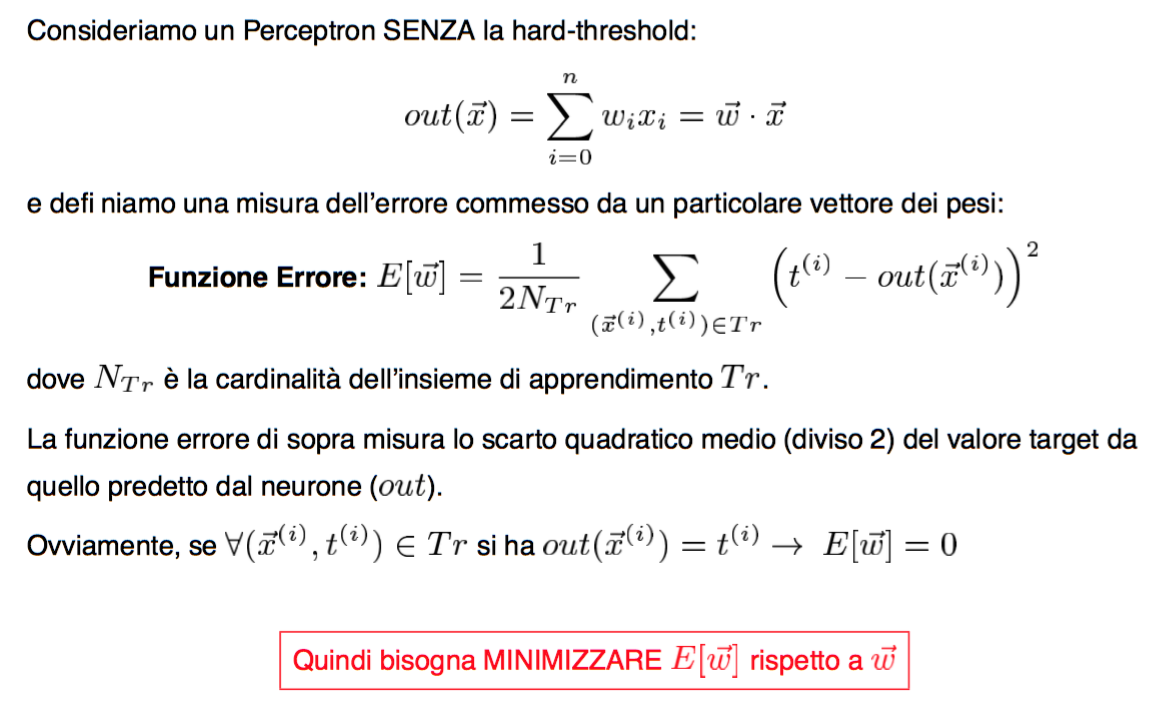
\includegraphics{./notes/immagini/l10-threshold.png}
\caption{}
\end{figure}

La funzione obiettivo da minimizzare è la \textbf{funzione errore}, la
quale rappresenta lo scarto quadratico medio del valore target predetto
dal neurone (\emph{funzione out}).

Dal momento che si tratta di una funzione derivabile è possibile
utilizzare la discessa di gradiente per raggiungere un minimo.

\begin{figure}[htbp]
\centering
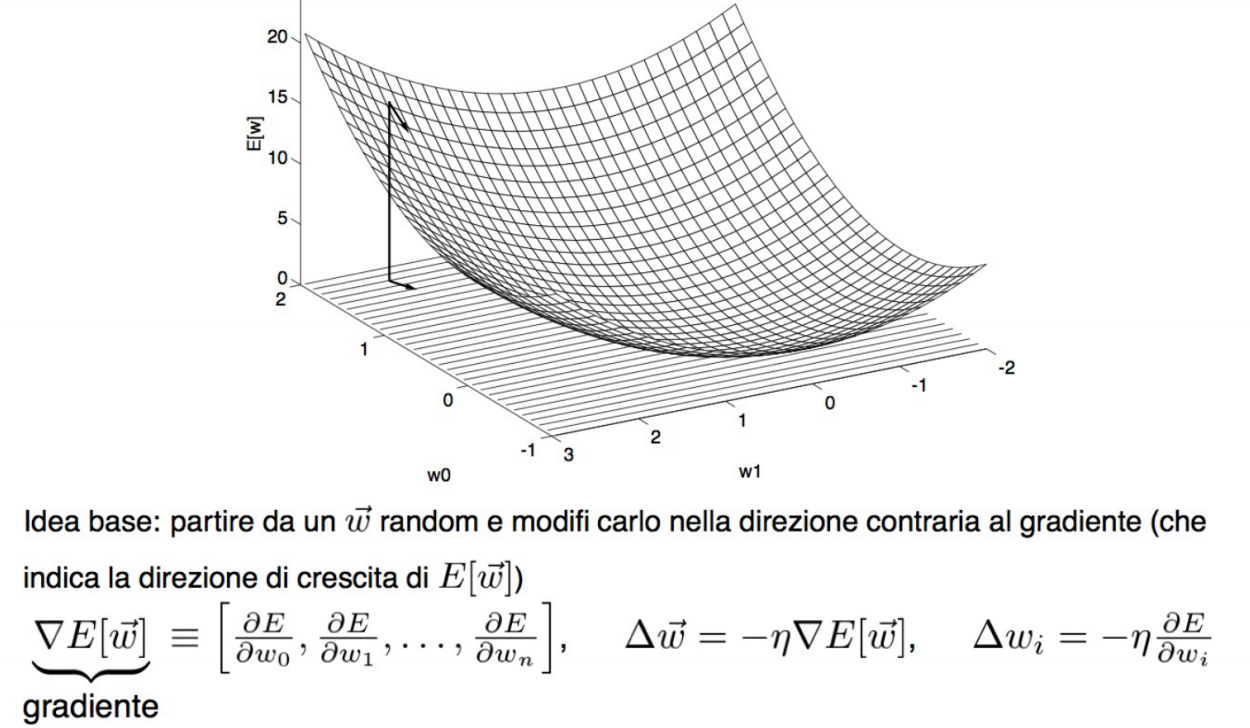
\includegraphics{./notes/immagini/l10-step.png}
\caption{}
\end{figure}

Il valore \emph{-η} è lo step con il quale mi sposto e prende il nome di
\textbf{learn rate}.

Per calcolare lo spostamento rispetto ad ogni \emph{wi} per minimizzare
la funzione obiettivo, vado a calcolare la derivata. Una volta calcolati
tutti i \emph{Δwi} posso andare a sommarli tra loro e successivamente
aggiornare il vettore \emph{w}.

La seguente serie di calcoli mostra come è possibile calcolare i
\emph{Δwi} per tutti gli esempi presenti nel training set. Viene usato
\emph{out(d)} per indicare il valore calcolato dalla rete per il
\emph{d}-esimo esempio del training set e \emph{t(d)} per indicare il
corretto valore della funzione target per lo stesso esempio.

In questo caso viene sempre considerata una rete di perceptron senza
hard-treshold e senza sigmoide.

\begin{figure}[htbp]
\centering
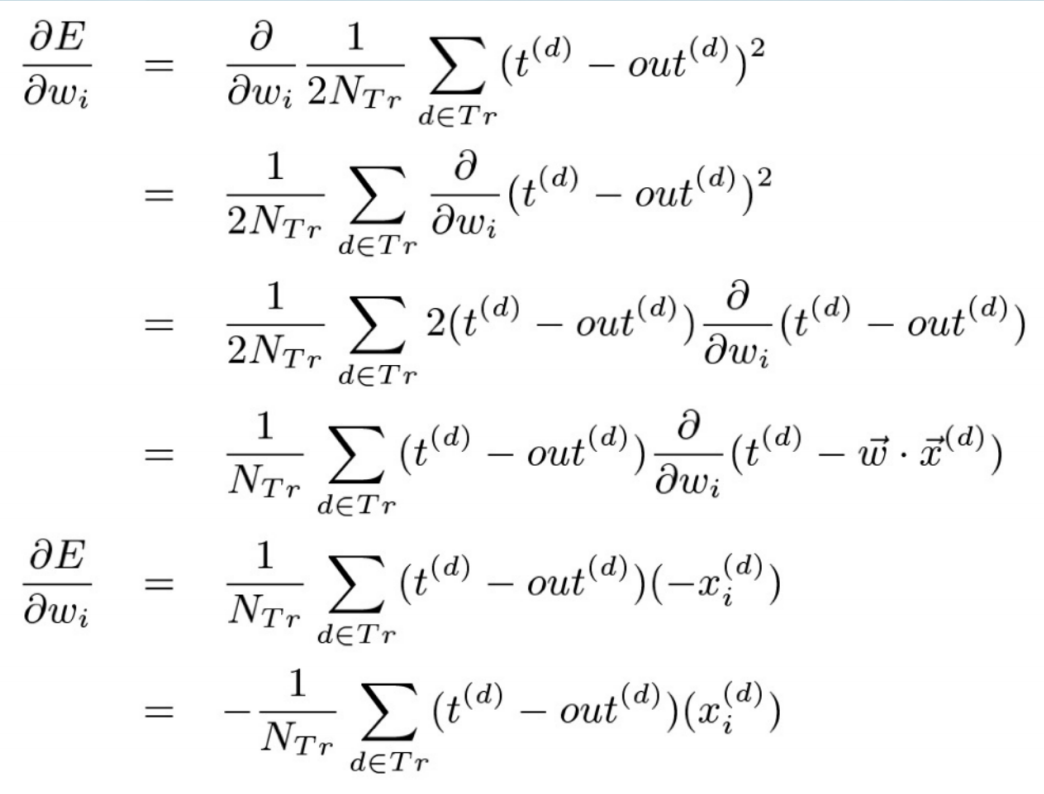
\includegraphics{./notes/immagini/l10-step-passaggi.png}
\caption{}
\end{figure}

\paragraph{Algoritmo di apprendimento}\label{algoritmo-di-apprendimento}

\emph{Δwi} rappresenta lo spostamento dal \emph{wi} iniziale.

\begin{figure}[htbp]
\centering
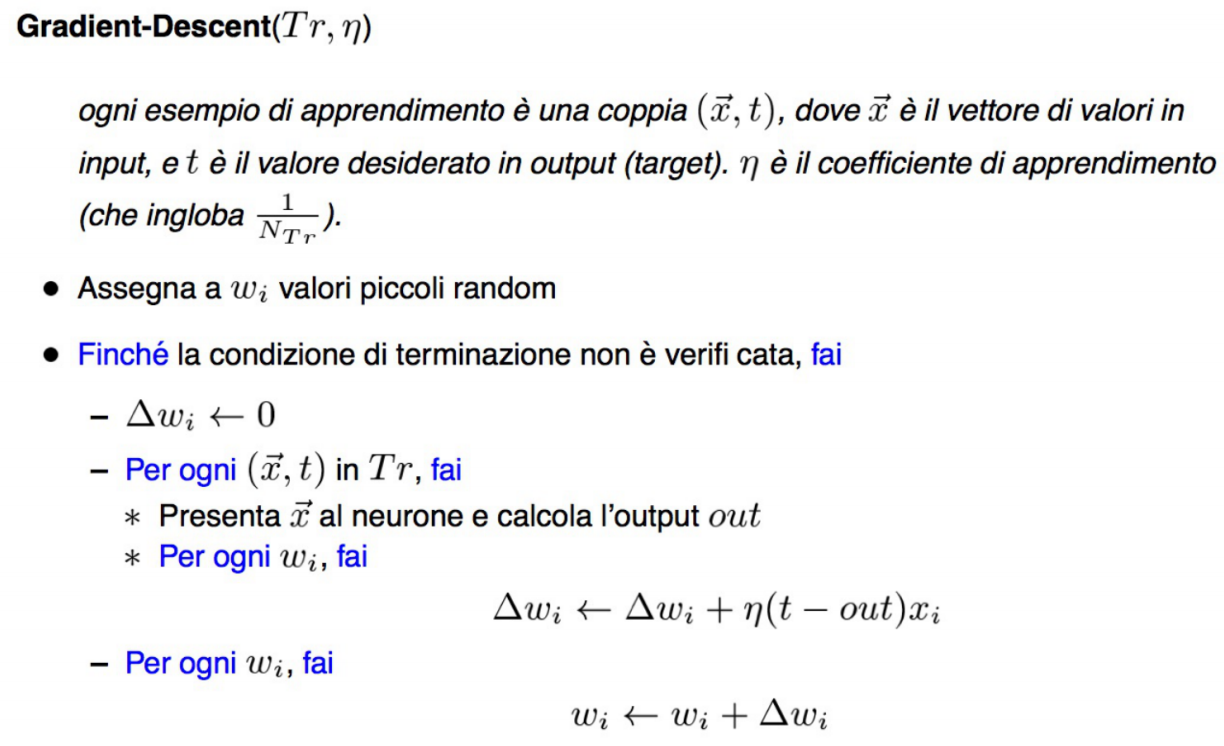
\includegraphics{./notes/immagini/l10-algoritmo-gradiente.png}
\caption{}
\end{figure}

In pratica prima viene esaminato tutti il training set per aggiornare i
vari \emph{Δwi}, una volta finito di esaminare il training set si
aggiornano i \emph{wi} e si ripete fino a che non si verifica una
condizione di stop.

Possono essere utilizzate varie condizioni di stop:

\begin{itemize}
\tightlist
\item
  \emph{E(w)} minore di una soglia prefissata
\item
  \emph{Δwi = 0 ∀i}
\item
  Il numero di iterazioni ha superato una soglia prefissata.
\end{itemize}

\subsubsection{Discesa di gradiente con
sigmoide}\label{discesa-di-gradiente-con-sigmoide}

\begin{figure}[htbp]
\centering
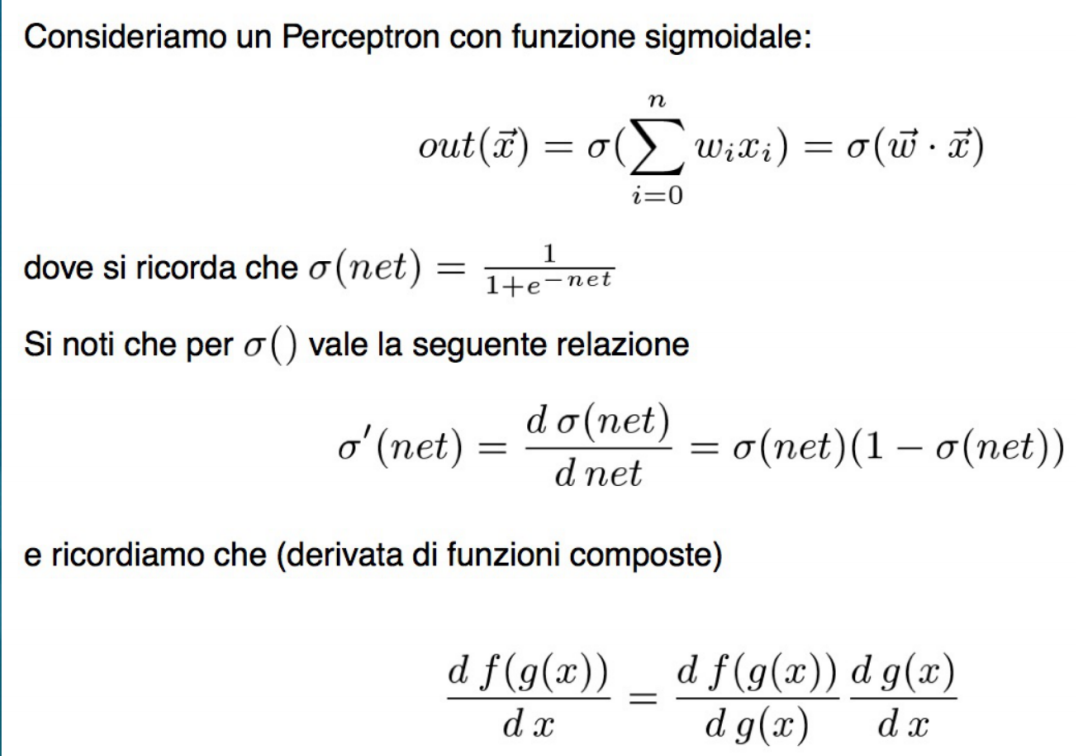
\includegraphics{./notes/immagini/l10-sigmoidale.png}
\caption{}
\end{figure}

In questo caso si può utilizzare lo stesso algoritmo di apprendimento
visto in precedenza, cambia però come vengono aggiornati i \emph{Δwi},
dal momento che bisona tenere in considerazione la derivata della
funzione sigmoidale.

\begin{figure}[htbp]
\centering
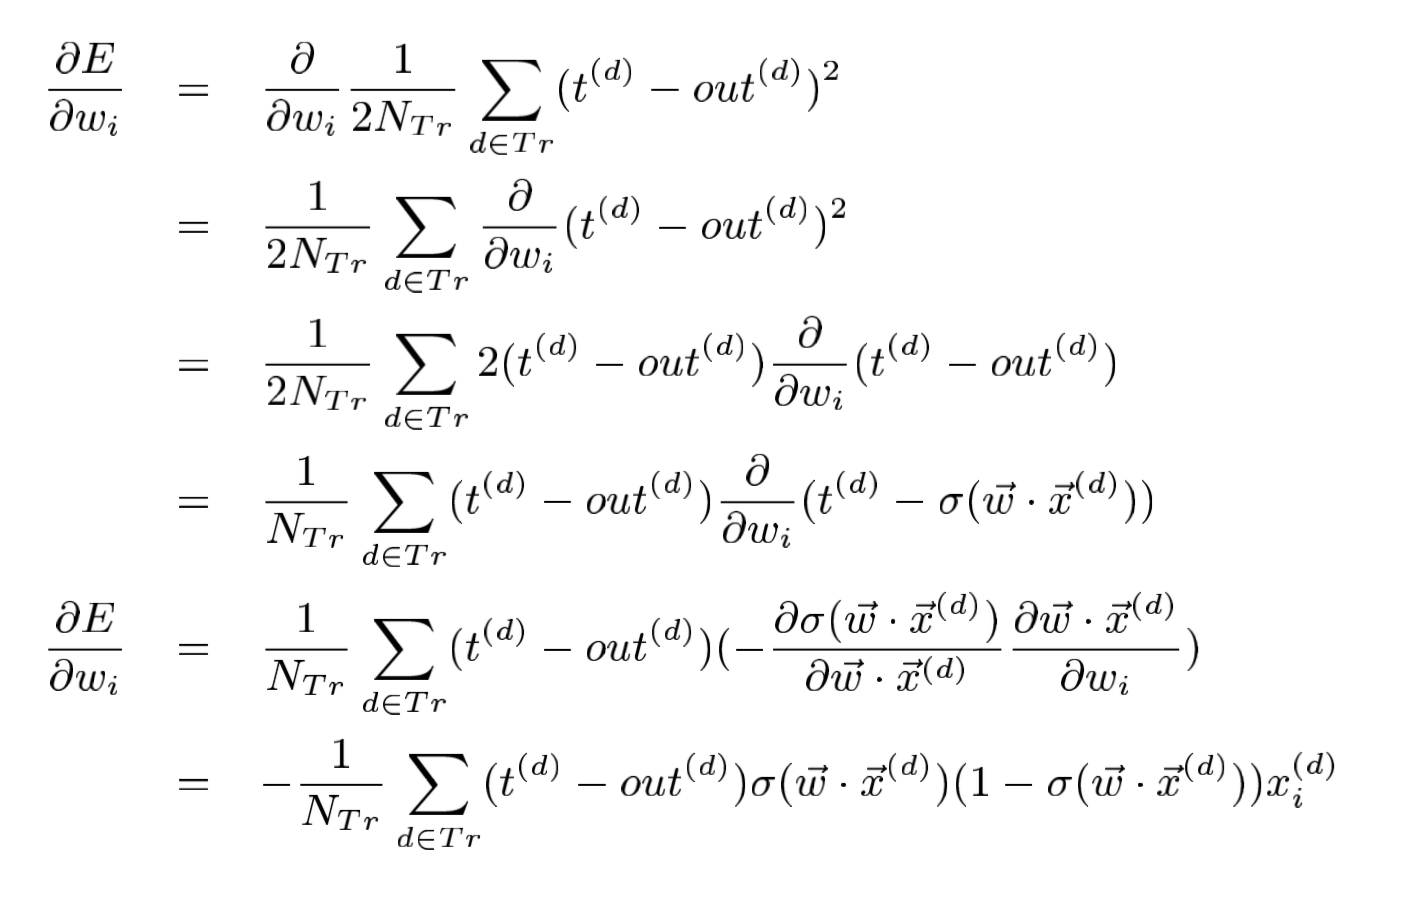
\includegraphics{./notes/immagini/l10-derivata-sigmoide.png}
\caption{}
\end{figure}

Nonostate la formula sembri molto minacciosa, i \emph{Δwi} sono uguali a
\emph{-η∂E / ∂wi}, cioè il learn rate moltiplicato per la derivata
appena calcolata.

\subsection{Rete di Perceptron}\label{rete-di-perceptron}

\begin{figure}[htbp]
\centering
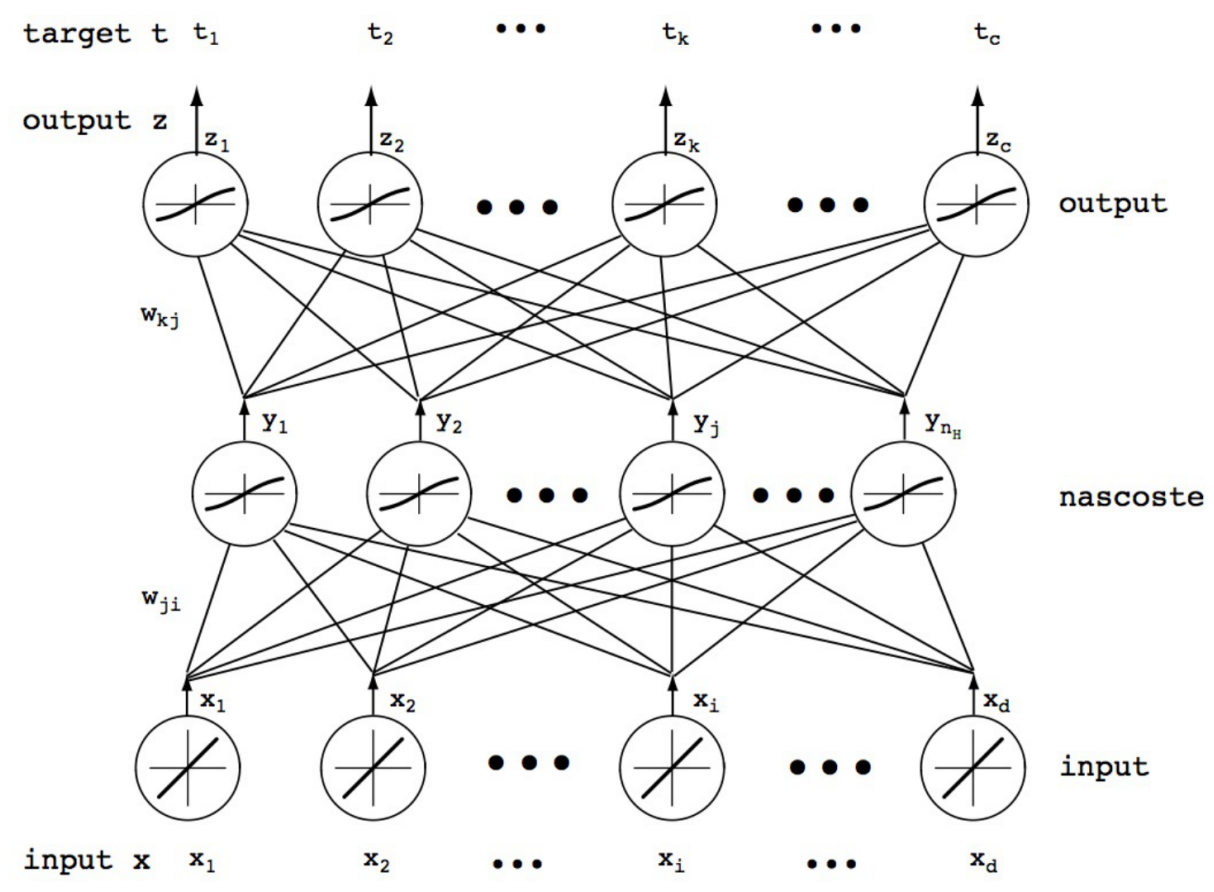
\includegraphics{./notes/immagini/l10-rete.png}
\caption{}
\end{figure}

\begin{figure}[htbp]
\centering
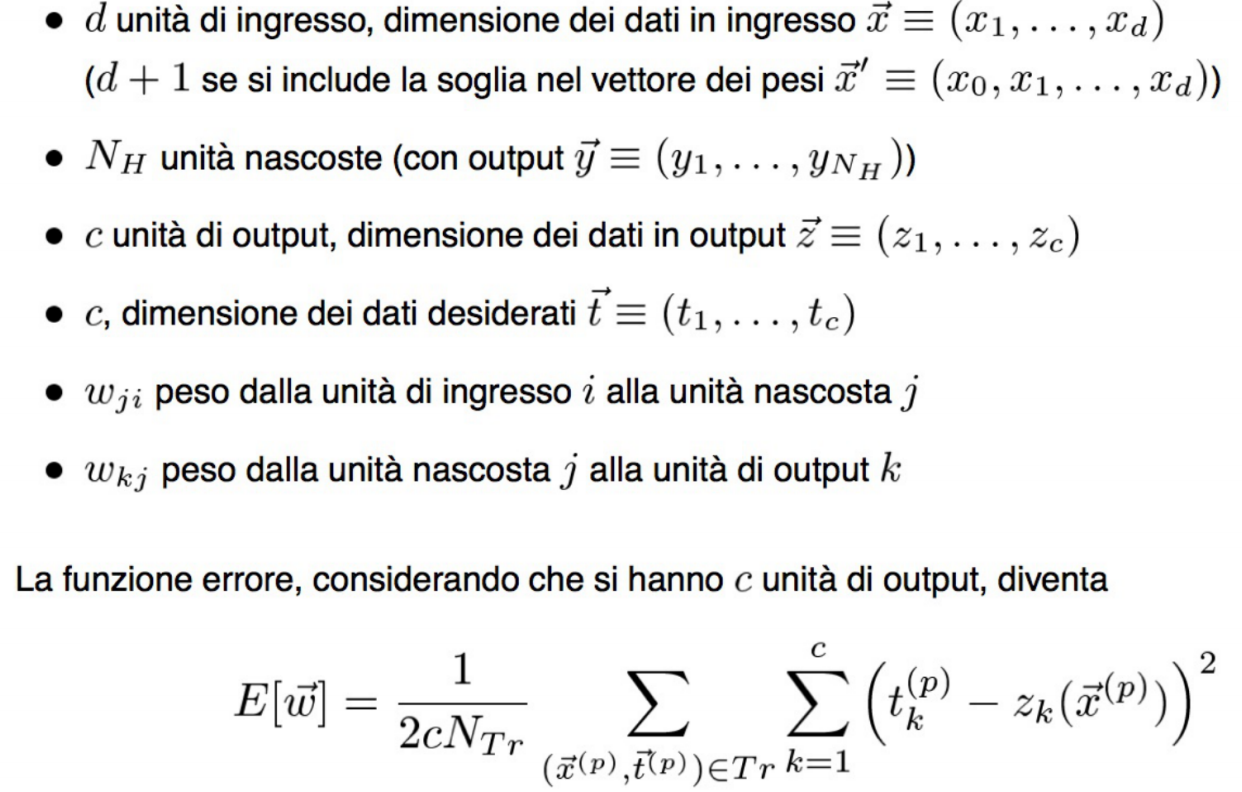
\includegraphics{./notes/immagini/l10-rete-parametri.png}
\caption{}
\end{figure}

E rappresenta l'errore quadratico medio di tutte le unità di output.

\subsubsection{Calcolo dei pesi per le unità di
output}\label{calcolo-dei-pesi-per-le-unituxe0-di-output}

Calcoliamo i pesi per le unità di output, considerando i livelli
nascosti come se fossero degli ingressi.

I \emph{wi} adesso diventano \emph{Δwk,j} perché i pesi vengono
calcolati per ogni collegamento da un'unità nascosta \emph{j} all'unità
di output \emph{k}.

\begin{figure}[htbp]
\centering
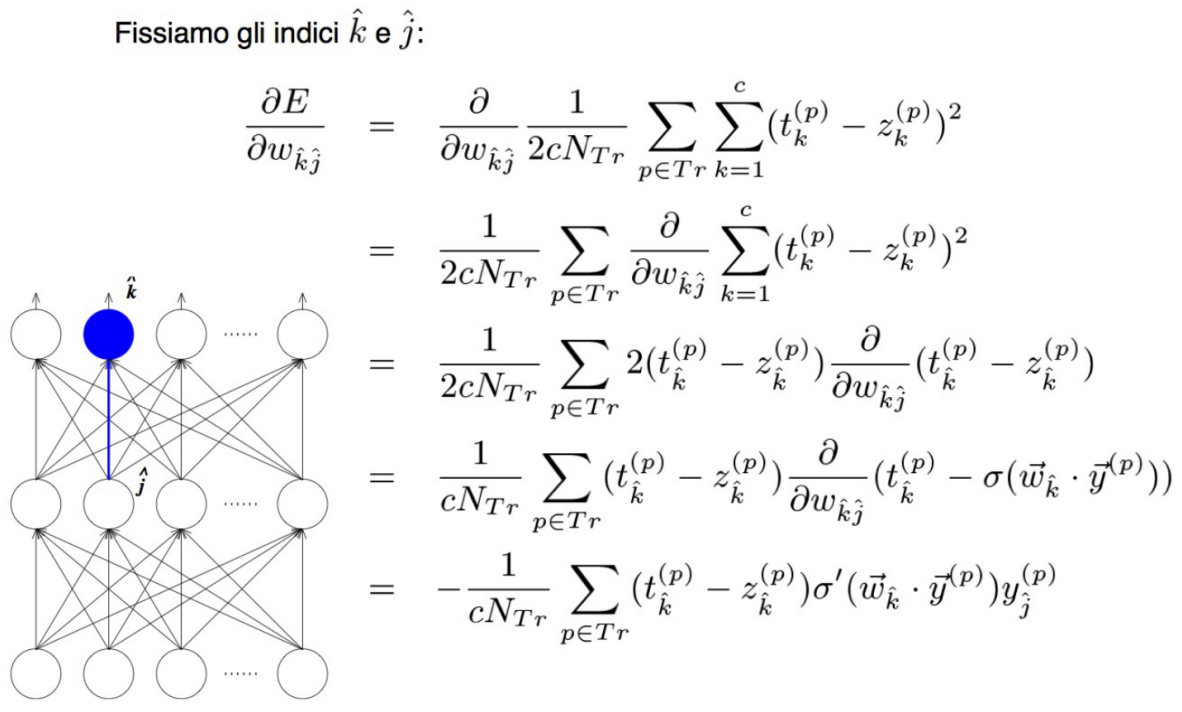
\includegraphics{./notes/immagini/l10-rete-output.png}
\caption{}
\end{figure}

Nel secondo passo sono state fatte due operazioni, prima viene tolta la
sommatoria, perché quando viene fatta la derivata della sommatoria c'è
un solo elemento diverso da ed è quello di indice \emph{k\^{}=k}.

\subsubsection{Calcolo dei pesi per le unità
nascoste}\label{calcolo-dei-pesi-per-le-unituxe0-nascoste}

\begin{figure}[htbp]
\centering
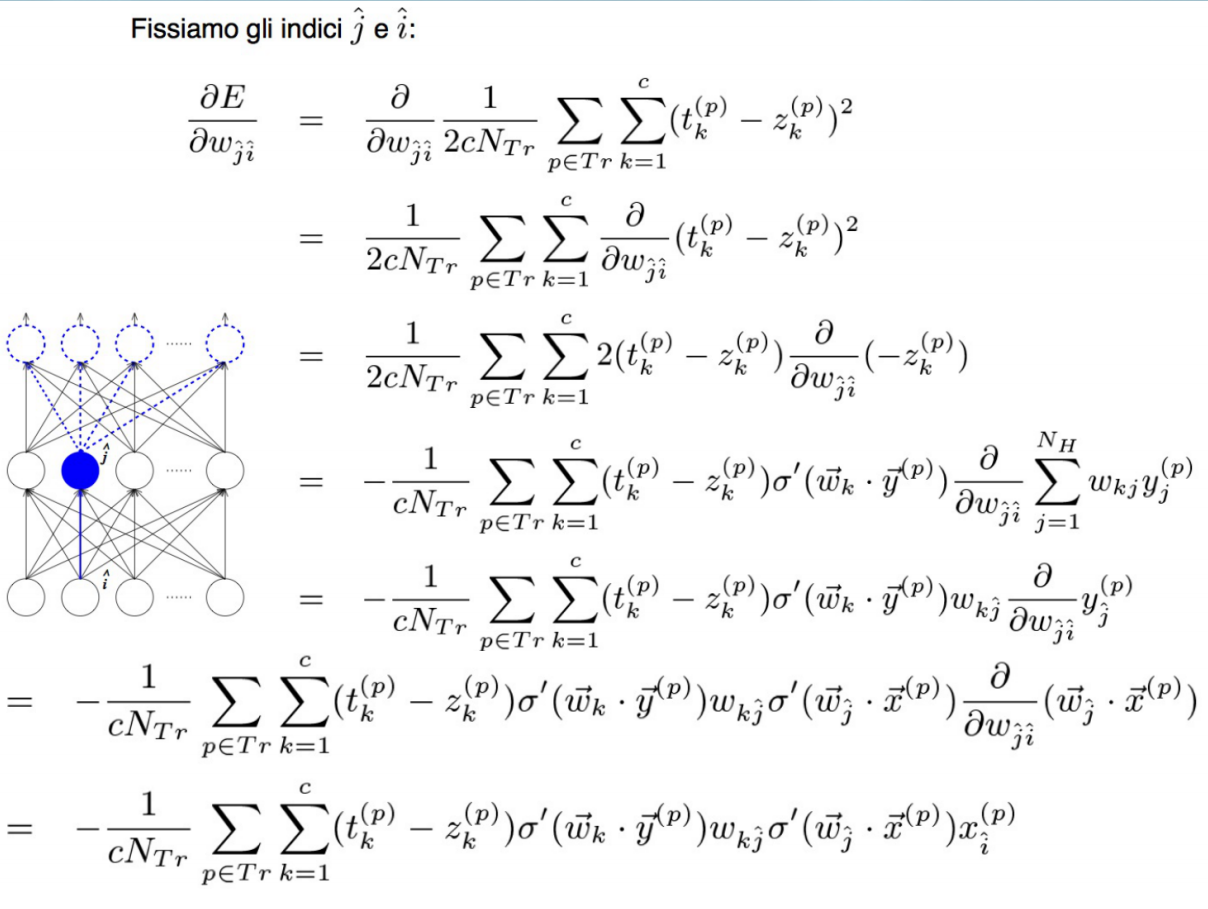
\includegraphics{./notes/immagini/l10-rete-input.png}
\caption{}
\end{figure}

\subsubsection{Algoritmo di
apprendimento}\label{algoritmo-di-apprendimento-1}

L'algoritmo di apprendimento lavora in due fasi: nella prima fase, detta
\textbf{feed forward}, viene forinto in input alla rete un esempio del
training set, in modo che questa possa provare a calcolare la funzione
target per l'esempio. Una volta calcolata si passa alla fase di
\textbf{backward progragation}, nella quale si aggiornarno i coefficenti
delle unità di output e delle unità nascoste in base alla correttezza o
meno della predizione. In questo caso l'apprendimento avviene a ritroso,
prima vengono aggiornati i coefficenti delle unità di output e poi
quelli dei livelli nascosti.

\begin{figure}[htbp]
\centering
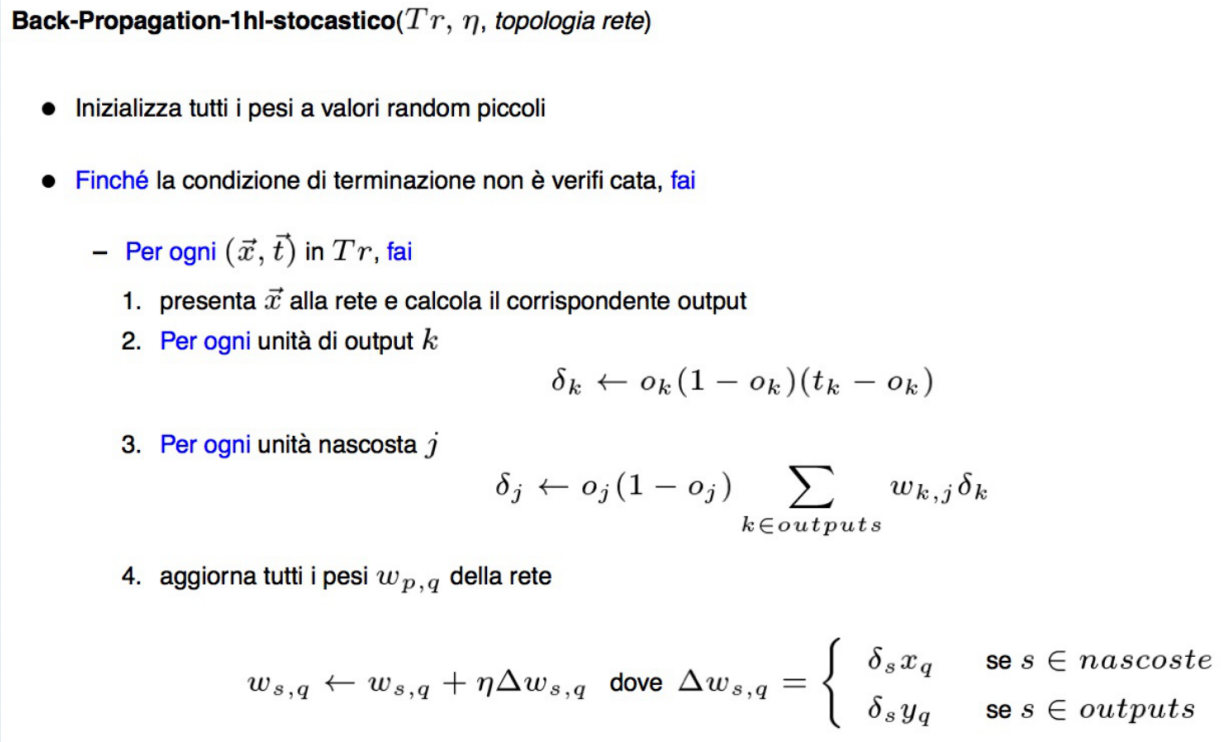
\includegraphics{./notes/immagini/l10-apprendimento-rete.png}
\caption{}
\end{figure}

Il passo 2 dell'algoritmo rappresenta il calcolo della differenza tra
l'output atteso e quello ottenuto, questo viene poi utilizzato per
aggiornare a ritroso i valori dei nodi interni (passo 3).

L'algoritmo prende il nome di \textbf{back propagation stocastico}
perché il valore dei \emph{Δwi} viene aggiornato subito dopo aver
valutato un esempio \emph{x} e non solamente dopo aver valutato tutti
gli esempi del training set.

Le possibili condizioni di terminazione sono le stesse che si hanno
quando c'è un solo neurone.
